\chapter{Diseño de la solución}\label{chap:Design}

Expuestas ya las distintas tecnologías que serán implementadas en nuestro trabajo, queda definir de qué modo estas serán utilizadas y cuál será su papel en la creación del proyecto.

\section{Diseño de la API}
La programación se rige por capas de abstracción. Partiendo de conceptos concretos se desarrolla una capa de abstracción haciendo uso de ellos que permite elevar el trato de elementos concretos un nivel por encima\cite{abstraction}. De esta forma ganamos en eficiencia y agilidad de escritura sin perder flexibilidad de desarrollo.

Una API, a grandes rasgos, no es más que una capa de abstracción sobre un lenguaje de programación o incluso sobre un framework del mismo. Comprende una serie de funciones que facilitan en mayor o menor medida trabajar sobre un cierto motivo. Como ejemplo de API famosa tenemos la de Google Maps, que contiene un compendio de métodos para JavaScript que permiten interactuar directamente con la plataforma de Google y crear nuestros programas jugando con ella\cite{googlemaps}. Podemos verlo como una biblioteca de funciones.

Como se ha citado previamente, GNS3 hace uso de una API REST (\textit{REpresentational State Transfer}). Esto es, mediante una serie de métodos (los conocidos GET, POST...) asociados a una URI concreta podemos interactuar vía web con una aplicación. La diferencia fundamental con otra clase de servicios web es que REST está orientado a recursos y no a métodos. Esto permite a la web utilizar comunicaciones sin estado, facilitando de este modo su escalabilidad\cite{REST}.

Aunque de increíble utilidad y ya veremos qué papel concreto juega en nuestro trabajo, necesitamos algo más para poder propiciar la interacción entre el simulador de redes y el videojuego. Necesitamos crear nuestra propia API que haga uso de la API REST de GNS3 y que defina métodos que permita a Unity interactuar con el SR de forma automática.

\subsection{Elección del lenguaje}

En pleno 2018 la cantidad de lenguajes de programación existentes roza el absurdo. Desde el tradicional C, pasando por el multifuncional Java, el sencillo Python o incluso los llamados lenguajes esotéricos como LOLCODE\cite{esotericlang}. De entre todos ellos nosotros elegiremos uno sobre el que trabajar. Esta decisión está condicionada, como es natural, por el motor de videojuegos a utilizar.

Ya que nuestra intención es que el MV sea capaz de establecer interacción con el SR, es necesario que la API a desarrollar esté escrita en un lenguaje con el que el propio motor sea capaz de trabajar. C\# parecía la opción más sensata. ¿Por qué? Las razones se exponen a continuación:

\begin{itemize}  
\item\textbf{Porque es el lenguaje más usado en Unity}. Unity admite varios lenguajes de programación con los que desarrollar los scripts asociados a los juegos. C++, usado en otros muchísimos otros motores de videojuegos como Unreal Engine, es uno de ellos. Aunque se trate de un lenguaje increíblemente potente y eficiente, su complejidad de uso es mucho mayor, ya que su nivel de abstracción es altamente inferior. JavaScript es otro de ellos, pero no es tan recomendable como C\#, pues entre otras razones, a diferencia de JS es fuertemente tipado\cite{unityinaction}. En general, Unity es el lenguaje usado por defecto en Unity y el recomendado por todos.
\item\textbf{Porque son más motores quienes lo utilizan}. Unity está en el podio de entre los motores de videojuegos más usados en el mundo. Como tal se convierte en un referente. El resto de motores miran hacia él y, si quieren atraer a nuevos programadores, tendrán que hacer de su incursión en el nuevo motor algo sencillo. Este es el caso de Godot Engine, que hace unos meses decidió incluir tal lenguaje entre los soportados\cite{godotcs}. Esto quiere decir que la API no solo podrá ser usada en juegos creados en Unity, si no que su terreno de juego se verá ampliado. CryEngine es otro de los motores que permiten el uso de C\# como lenguaje de scripting.
\item\textbf{Porque, ante todo, es un gran lenguaje}. C\#, similar en cuanto a sintaxis a Java, nació como respuesta a esta de la mano de Microsoft. Se trata de un lenguaje de propósito general aunque se use primordialmente para la construcción de aplicaciones para infraestructuras Windows. Es uno de los lenguajes que componen la plataforma .NET de Microsoft. Tal es su importancia que a día de hoy se posiciona como el cuarto lenguaje de programación más usado a nivel mundial\cite{csisfamous}.
\end{itemize}
Aclarada las razones, pasamos a analizar el uso que le daremos a este lenguaje.

\subsection{La API}
Antes de desarrollar la API es necesario reflexionar sobre la forma que tendrá. Para dar soluciones, tenemos que plantearnos antes las preguntas adecuadas:
\subsubsection[''Interacción con GNS3'']{¿Cómo debe interactuar con el simulador?}
Como ya se dijo con anterioridad, GNS3 crea un servidor en el equipo desde el que se ejecuta. Este servidor acepta peticiones REST, creando así una suerte de interacción con el programa sin necesidad de poner las manos en él de forma directa. Se abre de esta forma al mundo del scripting y así a nosotros para crear un conjunto de métodos que faciliten su acceso y gestión.

Tratándose de una API REST, lo único que no es necesario para la conexión es un cliente web. Será pues sobre esto sobre lo que se base primordialmente la relación entre nuestra librería y el simulador de redes como tal. A continuación veremos que no será necesario el uso de alguna tecnología más.


\subsubsection[''Acceso a la API'']{¿Cómo queremos que interactúe con el exterior?}


\subsubsection[''Utilidad'']{Más importante aún, ¿qué queremos que haga?}

\subsection{Estructura de clases}
\begin{figure}[h]
  \centering
  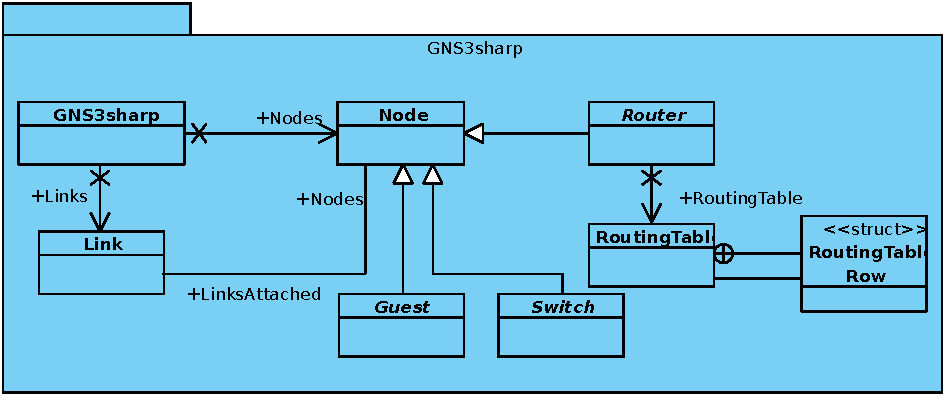
\includegraphics{imagenes/diagrama_api1}
  \caption{Boceto de diagrama UML de la API}
  \label{fig:diagrama_api1}
\end{figure}
\subsubsection[''La clase principal'']{GNS3sharp, la clase principal}
\subsubsection{Nodes}
\subsubsection{Links}
\subsubsection{Otras clases}
\subsection{GitHub y la comunidad}


\section{Diseño del videojuego}
\subsection{Interacción con el simulador}
\subsection{Propuestas de modelo de videojuego}



